\documentclass[]{article}
\usepackage{graphicx}

%opening
\title{Assignment 1 CDA}
\author{Tim van Rossum, 4246306\\
	Michiel Doesburg,}

\begin{document}

\maketitle

\section{A visualization of the data}
For the visualization part of this assignment, we first started out by making bar plots of different kinds, but eventually settled  for the scatterplot as seen in figure 1. This scatterplot uses the amount of Eurocent spent per transaction, to allow for better comparisons to be made, as there were five different currencies in the dataset. Exchange rates of April 25, 2018 were used. As can be seen from the scatterplot, there are basically no fraudulent transactions where more than 800 Euro was spent, while there are benign transactions where more than 800 Euro was spent. Also, there are significantly more fraudulent transactions originating from Mexico and Australia than there are from the rest of the world. 
\begin{figure}[h!]
	\centering
	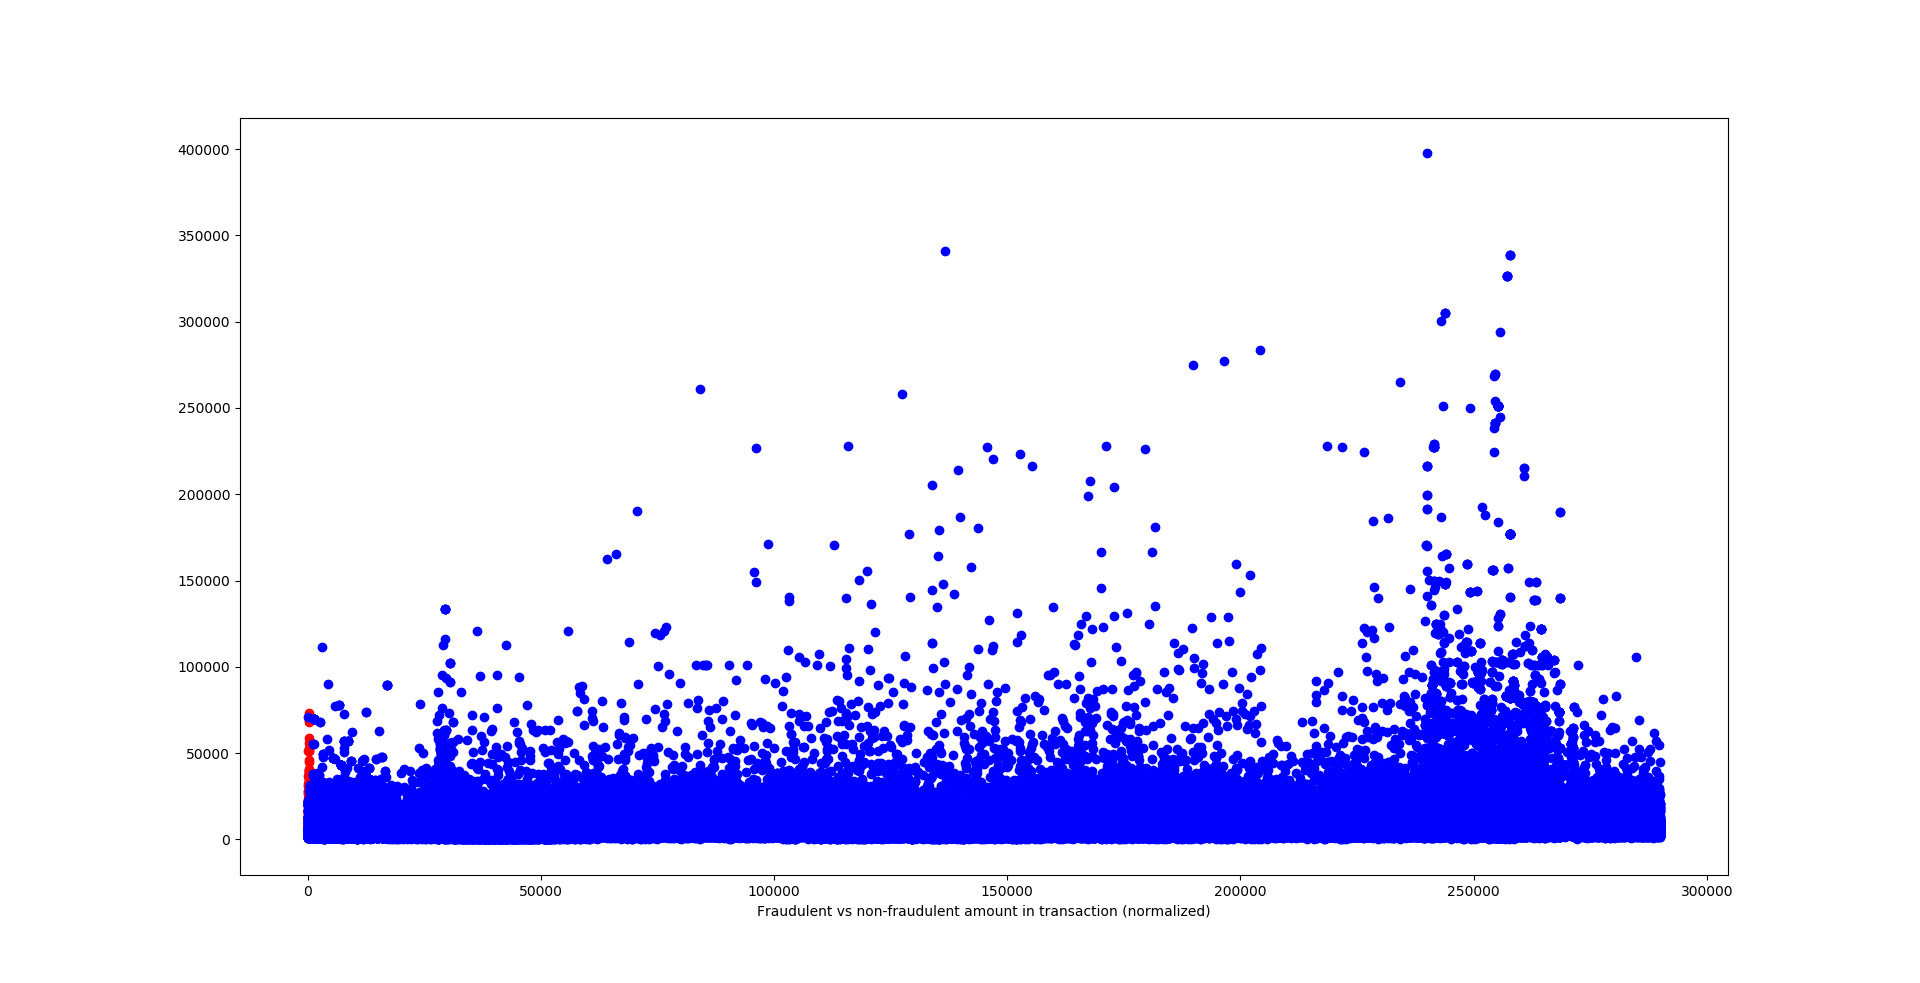
\includegraphics[scale = 0.25]{Visualizations/fraud_vs_nonfraud_better}
	\caption{A scatterplot of the amount of money spent in the sampled transactions. A red dot indicates a fraudulent transaction (these are only at the very left of the plot due to very little fraudulent transactions existing), while a blue dot indicates a benign transaction.}
\end{figure}
\clearpage
\section{Applying SMOTE to the data}
Because we used Python for this assignment with \texttt{scikit-learn}, we used SMOTE as implemented in the package \texttt{imblearn}. The \texttt{fraud\_detection.py} script already preprocessed the data in such a way that applying SMOTE to it was very easy, as the implementation only needed the data and the class labels, and both were already generated by the script. The general steps of preprocessing are: 
\begin{itemize}
	\item Remove data with the "Refused" label (as that is data where we cannot be certain whether or not it is fraudulent)
	\item Remove the ID and booking date of the transaction, as these are not necessary.
	\item Transform the mail identifiers, IP identifiers etc. to simply the number that they use.
\end{itemize}
The classifiers that we used were the random forest classifier, the 5-NN classifier, and the logistic classifier. These were chosen to represent both linear and non-linear classifiers, as well as parametric and non-parametric classifiers (as NN is deemed a non-parametric classifier). The ROC curves are shown in figure 2.
\begin{figure}[h!]
	\centering
	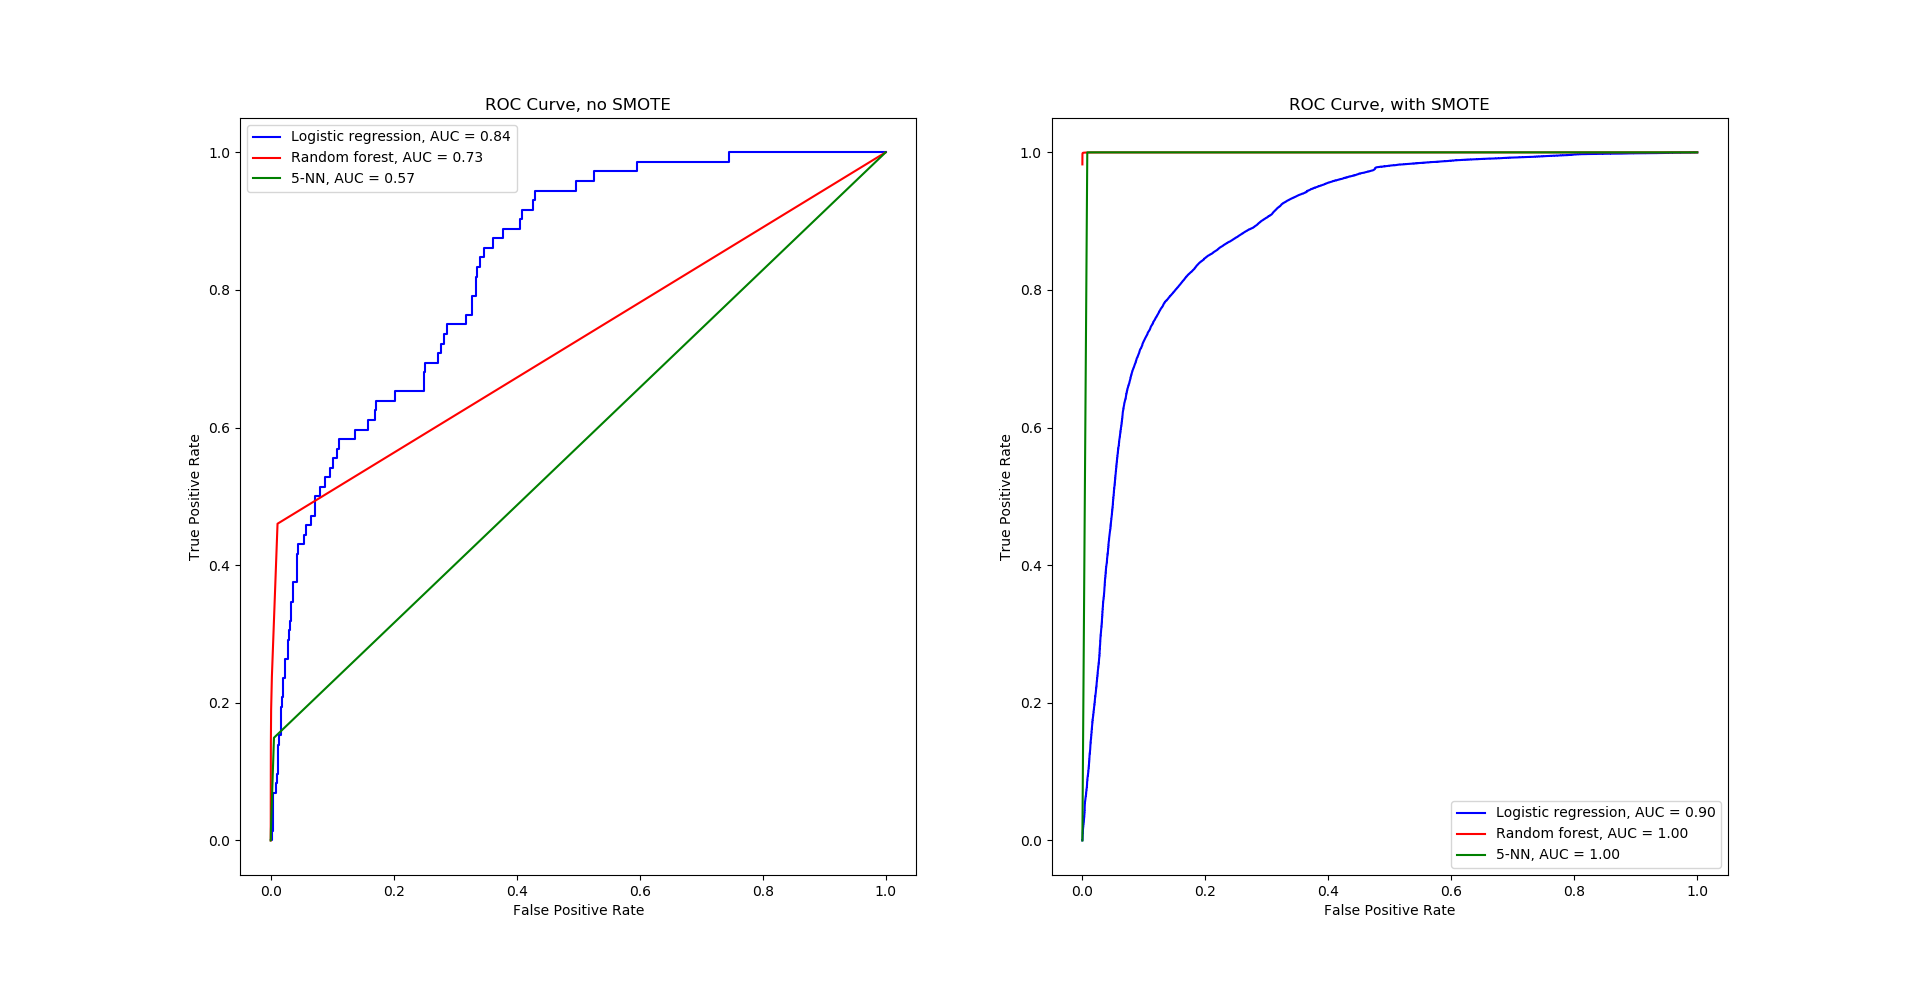
\includegraphics[scale = 0.25]{Visualizations/ROC_curves}
	\caption{Caption of ROC curves.}
\end{figure}
\clearpage
\section{The black box and white box classifier}
For the white box classifier, we will use the following decision rules to determine whether or not a transaction is fraudulent:
\begin{itemize}
	\item The transaction originates from either Mexico or Australia (as these two countries have about two-third of the total fraudulent transactions).
	\item The card issuer identifier is between 401795 and 558320, both inclusive. This is the range in which fraud was detected.
	\item The card type used was mccredit, visaclassic or visadebit. These three card types are used in about two thirds of the fraud cases.
	\item In the case of Australia, for a transaction to be classified as fraudulent, the currency used must be the Australian dollar, the merchant's webshop value should be APACAccount, the the card verification code must be supplied, the amount spent must be between 250 AUD and 350 AUD, the interaction should be via E-commerce, and the CVC response code should be 0.
	\item In the case of Mexico, for a transaction to be classified as fraudulent, the currency used must be the Mexican peso, the merchant's webshop value should be MexicoAccount.
\end{itemize}
For the black box classifier, we will be using the random forest classifier, as this classifier tended to perform better, especially on SMOTEd data. It is also a classifier that has been shown to perform better in the papers
\end{document}
